\subsection{Version control system}

\subsubsection{Tortoise SVN}

\subsubsection{GitHub}

GitHub is a web-based hosting service for software development projects that use the Git revision control system. GitHub offers both commercial plans and free accounts for open source projects.\newline

Collaboration on Github is not complicated but also not intuitively clear for beginners because not all parts of the workflow are incorporated into the Github user interface. This description describes the structure of collaboration between the contributors and the maintainers of a project that is hosted on github. For every step in the workflow the respective git commands are given for reference.

\begin{figure}[github]
	\centering
	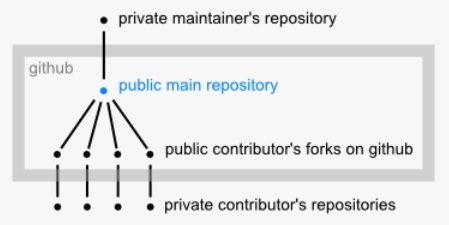
\includegraphics[width=0.8\textwidth]{prestudy/github.jpg}
	\caption{Distributed setup of git repositories}
	\label{fig:usecase}
\end{figure}